\documentclass{sageep}
\usepackage{lipsum}
\usepackage{graphicx}
\begin{document}
\title{New Green Technology: A Method of Extracting Sun Energy From
  Fresh Cucumbers} 
\author{Sam U. Llaun, Academy of Lagado, Lagado, Balnibarbi}
\author{James Incandenza, Interdependence University, Boston, MA}
\maketitle

\section{Abstract}

\lipsum[1]

\section{Discussion}



\subsection{First Subsection}

The use of PostScript fonts is described in
\cite{Schmidt04:PSNFSS9.2}.  The popular \LaTeX{} manual is
\cite{Lamport94}.  The use of \TeX{} in scientific
publishing\footnote{As well as in other publishing fields} was
discussed in \cite{Flynn01:TeXMassMarket}. 


\begin{figure}[bhp]
  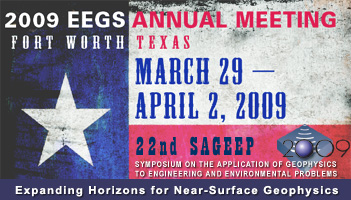
\includegraphics{sageep_graphic2009}
  \caption{SAGEEP Meeting}
  \label{fig:sageep}
\end{figure}

\begin{table}[htbp]
  \caption{North American Paper Sizes}
  \label{tab:paper}
  \begin{tabular}{lll}
    \hline
    Size & in $\times$ in &mm $\times$ mm\\
    \hline
    Letter &8.5 $\times$ 11 &216 $\times$ 279\\
    Legal &8.5 $\times$ 14 &216 $\times$ 356\\
    Junior Legal &8 x 5 &\\
    Ledger &17 $\times$ 11 &432 $\times$ 279\\
    Tabloid &11 $\times$ 17 &279 $\times$ 432\\
    \hline
  \end{tabular}
\end{table}


\lipsum[2-5]


\subsection{Second Subsection}

\lipsum[5-8]

\section{Conclusions}

\lipsum[9-10]

\bibliography{sageep}
\bibliographystyle{sageep}

\end{document}
